\documentclass{ximera}

\input{../preamble.tex}

\title[Dig-In:]{A tale of three integrals}

\begin{document}
\begin{abstract}
  At this point we have three ``different'' integrals. 
\end{abstract}
\maketitle

At this point we have three different ``integrals.'' Let's see if we
can sort out the differences.

\section{Indefinite integrals}

An indefinite integral, also called an \dfn{antiderivative} computes
classes of functions:
\[
\int f(x) \d x = ``\text{a class of functions whose derivative is $f$''}
\]
Here there are no limits of integration, and your answer will have a
``$+C$'' at the end. Pay attention to the notation:
\begin{image}
  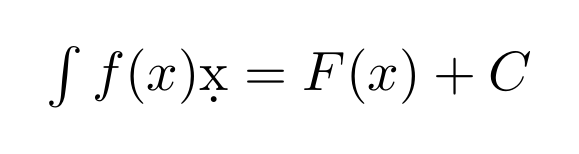
\begin{tikzpicture}[scale=2,every node/.style={transform shape}]
    \node at (0,0) {
      $\int f(x) \d x = F(x) + C$
      };
  \end{tikzpicture}
\end{image}
Where $F'(x) = f(x)$.
\begin{explanation}%%%BADBAD I would like no environment here.
  Indefinite integrals
  \wordChoice{\choice{have}\choice[correct]{do not have}} limits of
  integration, and they compute \wordChoice{\choice{signed
      area}\choice{an antiderivative}\choice[correct]{a class
      of antiderivatives}}.
\end{explanation}

\begin{question}
  Two students, say Devyn and Riley, are working with the following
  indefinite integral:
  \[
  \int \sin(x)\cos(x)\d x
  \]
  Devyn computes the integral as
  \[
  \int \sin(x)\cos(x)\d x = -\frac{1}{2}\cos^2(x) + C
  \]
  and Riley computes the integral as
  \[
  \int \sin(x)\cos(x)\d x = \frac{1}{2}\sin^2(x) + C.
  \]
  Which student is correct?
  \begin{multipleChoice}
    \choice{Devyn is correct}
    \choice{Riley is correct}
    \choice[correct]{Both students are correct}
    \choice{Neither student is correct}
  \end{multipleChoice}
  \begin{feedback}
    Both students are correct! The seeming discrepancy arises from the
    fact that the ``+C'' in each case is \textit{different}!
  \end{feedback}
\end{question}





\section{Accumulation functions}

An \dfn{accumulation function}, also called an \dfn{area function}
computes accumulated area:
\[
\int_a^x f(t) \d t = ``\text{a function $F$ whose derivative is $f$''}
\]
This is a function of $x$ whose derivative is $f$, with the additional
property that $F(a)=0$.  Pay attention to the notation:
\begin{image}
  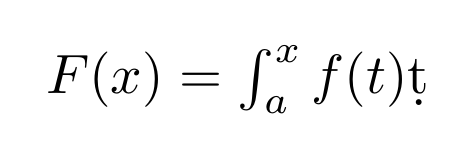
\begin{tikzpicture}[scale=2,every node/.style={transform shape}]
    \node at (0,0) {
      $F(x)=\int_a^x f(t) \d t$
      };
  \end{tikzpicture}
\end{image}
Where $F'(x) = f(x)$.
\begin{explanation}%%%BADBAD I would like no environment here.
  Accumulation functions \wordChoice{\choice[correct]{have}\choice{do
      not have}} limits of integration, and they compute
  \wordChoice{\choice{signed area}\choice[correct]{an antiderivative}\choice{a class of antiderivatives}}.
\end{explanation}
\begin{question}
  True or false: There exists a function $f$ such that 
  \[
  \int_0^x f(t) \d t = \cos(x)
  \]
  \begin{multipleChoice}
    \choice{true}
    \choice[correct]{false}
  \end{multipleChoice}
  \begin{feedback}
    Let
    \[
    F(x) = \int_0^x f(t) \d t,
    \]
    this is an accumulation function and $F(0) = 0$, since no area is
    accumulated yet. However, $\cos(0) =1$. Hence there can be no such
    function $f$. On the other hand, there is a function $g$ with
     \[
     \int_0^x g(t) \d t = \cos(x)-1
     \]
     namely, $g(x) = \cos(x)$. This subtlety arises from the fact that an
     accumulation function
     \[
     F(x) = \int_a^x f(t) \d t
     \]
     gives a \textbf{specific} antiderivative of $f$, the one that
     when evaluated at $x=a$ is zero.
  \end{feedback}
\end{question}










\section{Definite integrals}

A \dfn{definite integral} computes signed area:
\[
\int_a^b f(x) \d x = ``\text{the signed area between the $x$-axis and $f$}''
\]
Here we always have limits of integration, both of which are
numbers. Moreover, definite integrals have definite values, the signed
area between $f$ and the $x$-axis. Pay attention to the notation:
\begin{image}
  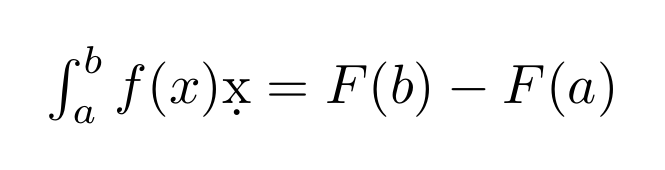
\begin{tikzpicture}[scale=2,every node/.style={transform shape}]
    \node at (0,0) {
      $\int_a^b f(x) \d x = F(b)-F(a)$
      };
  \end{tikzpicture}
\end{image}
Where $F'(x) = f(x)$.
\begin{explanation}%%%BADBAD I would like no environment here.
  Definite integrals \wordChoice{\choice[correct]{have}\choice{do
      not have}} limits of integration, and they compute
  \wordChoice{\choice[correct]{signed area}\choice{an antiderivative}\choice{a class of antiderivatives}}.
\end{explanation}

\begin{question}
  Consider
  \[
  f(x) =
  \begin{cases}
    -2  &\text{if $x< 1$,}\\
    2 &\text{if $x\ge 1$.}
  \end{cases}
  \]
  If we compute an antiderivative of $f$, we find
  \[
  F(x) =
  \begin{cases}
    -2x  &\text{if $x< 1$,}\\
    2x &\text{if $x\ge 1$.}
  \end{cases}
  \]
  Is it correct to say
  \begin{align*}
    \int_0^1 f(x) \d x &= \eval{F(x)}_0^1 \\
    &=F(1) - F(0)\\
    &=2 ?
  \end{align*}
  \begin{multipleChoice}
    \choice{yes}
    \choice[correct]{no}
  \end{multipleChoice}
  \begin{feedback}
    Perhaps the first thing to do would be to attempt to analyze this
    geometrically. Here we see our function and the signed area
    computed by the integral:
    \begin{image}
      \begin{tikzpicture}
	\begin{axis}[
            domain=-.5:1.5,
            axis lines =middle, xlabel=$x$, ylabel=$y$,
            every axis y label/.style={at=(current axis.above origin),anchor=south},
            every axis x label/.style={at=(current axis.right of origin),anchor=west},
            clip=false,
            %axis on top,
          ]
          \addplot [draw=none,
            fill=fillp, domain=0:1] {-2} \closedcycle;
          \addplot [textColor, very thin, domain=(0:1.5)] {0}; % puts the axis back, axis on top clobbers our open holes
          \addplot [textColor, very thin] plot coordinates {(0,0) (0,2)}; % puts the axis back, axis on top clobbers our open holes
	  \addplot [very thick, penColor, domain=(-.5:1)] {-2};
          \addplot [very thick, penColor, domain=(1:1.5)] {2};
          \addplot[color=penColor,fill=penColor,only marks,mark=*] coordinates{(1,2)};  %% closed hole          
          \addplot[color=penColor,fill=background,only marks,mark=*] coordinates{(1,-2)};  %% open hole
        \end{axis}
      \end{tikzpicture}
    \end{image}
    From the graph above, we can see that
    \[
    \int_0^1 f(x) \d x =-2.
    \]
    So now the question is, ``what went wrong'' above? In this case
    our function $f$ is \textbf{not} continuous! For The Fundamental
    Theorem of Calculus to apply, the integrand \textbf{must} be
    continuous on the interval that one is integrating on. If this is
    not the case, the fundamental theorem may or may not yield valid
    results.
  \end{feedback}
\end{question}

\end{document}
